\documentclass[letterpaper,twocolumn,10pt]{article}

\usepackage{tikz}
\usepackage{amsmath}
\usepackage{graphicx}
\usepackage{float}
\usepackage{lipsum}
\usepackage{sidecap}
\usepackage{hyperref}
\usepackage{xcolor}
\usepackage{listings}

\usepackage{titling}

%\usepackage[left=0.5in,right=0.5in, bottom=0.5in]{geometry}
\setlength{\droptitle}{-0.6in}
\usepackage[margin=0.5in]{geometry}



%-------------------------------------------------------------------------------
\begin{document}
% -------------------------------------------------------------------------------

\date{} % avoid printing of date

\title{Optimising a Stencil Code for a single CPU}

\author{
  {\rm Jan Fecht / rr19492}\\
  Introduction to High Performance Computing}

\maketitle


% -------------------------------------------------------------------------------
\section*{Introduction}
% -------------------------------------------------------------------------------
The program to be optimised consists of a simple convolution kernel applied on a chessboard-pattern image.
The user can specify the width $nx$ and the height $ny$ of the image and furthermore
the number of times $k$ that the stencil is applied. All of these parameters are passed on the command line to the program, except for $k$ which is passed as $k/2$ (niters) instead.

For comparing and evaluating the effect of
the algorithmic optimisation, the final version of the code was benchmarked
and compared to the final version without the optimisation. The reason for this is
that the optimisation was introduced rather late which makes it hard
to apply the optimisation seperatly onto the original version as a lot of code rewriting
would be necessary.
Memory- and vectorization-related optimisations, on the other hand, are introduced in a
progressive manner, starting with the original version.

Measured times were determined by taking the average of 50 runs
on the University's \textit{Blue Crystal 4} supercomputer (\textit{bc4}). The times for
the original version were taken from the official repository
\footnote{\url{https://github.com/UoB-HPC/intro-hpc-stencil/}} instead, as running it 100 times would have been impractical.

The speedup of the final version can be seen in Table~\ref{tab:final}.

\vspace{0.10in}

\textbf{Disclaimer} The optimisations applied were neither introduced
in the order nor grouped together as they are described in this report. Rather, the 
whole optimisation process was iterative because new ideas and adaptations to new
circumstances were necessary. To see the full progression, run \texttt{git log} in the root
of the project directory.

\begin{table}[ht]
	\vspace{-0.2in}
	\caption{Original compared to final version ($k=200$).}
	\begin{tabular}{c c c c}
		 image size & original & final & speedup \\
		 \hline
		1024 x 1024 & 5.908341s   & 0.01626971s & 363.15\\
		4096 x 4096 & 130.196475s & 0.02686471s & 4846.38\\
		8000 x 8000 & 561.118133s & 0.0451399s & 12430.65\\
	\end{tabular}
	\label{tab:final}
	\vspace{-0.3in}
\end{table}

% -------------------------------------------------------------------------------
\section*{Algorithm}
% -------------------------------------------------------------------------------
The chessboard pattern contains a high degree of symmetry and by applying the stencil code
to all points the original code performs an excess of redundant computations.
The number of floating point operations lies in $\Theta(nx * ny * k)$
as the number of points to be stenciled is $nx * ny$.
To reduce this number drastically, one can stencil only small parts of the image and apply
these precomputed parts to the whole image by copying and possibly mirroring or inverting them.
The specific parts that need to be precomputed can be seen
in Figure~\ref{fig:board}. The center part in red cannot
be applied to the whole image but only to the center in transparent red.
The reason for this lies in the way the borders are stenciled in the original version. It assumes
that there is an invisible black border around the field. This leads to a slightly darker border
which affects all pixels in a range of $k$ around the border. This is marked as the
green, blue and yellow parts in Figure~\ref{fig:board}. Furthermore, we also need to include some parts of the center when computing the border and corner parts because the points closest to the center will also be affected by the center itself. That is why we are using $k'$ instead of $k$ in Table~\ref{tab:numstencil}.

\begin{figure}[t]
	\begin{center}
	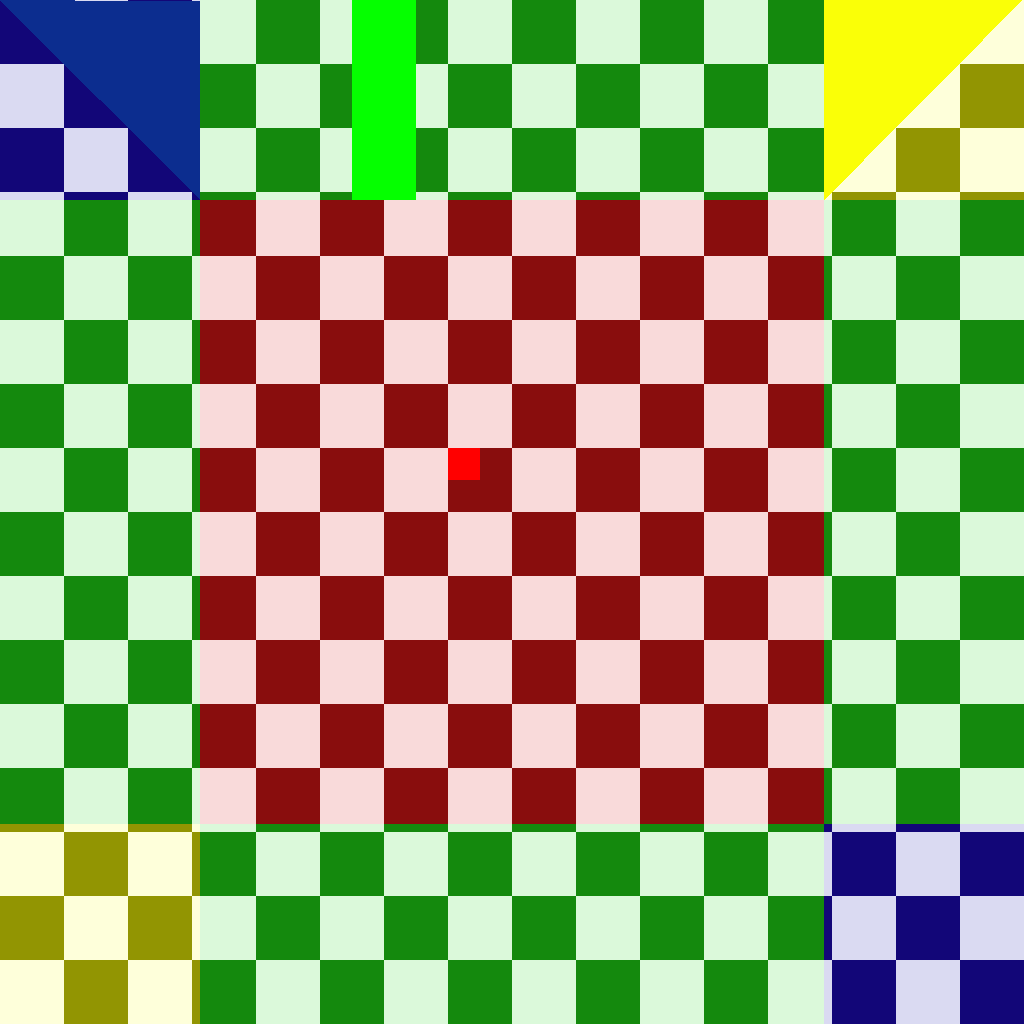
\includegraphics[width=150pt]{res/stencil_colored_with_prec}
	\caption{Coloured 1024 x 1024 pattern assumming $k = 200$. Areas that need to be precomputed are opaque.}
	\label{fig:board}
	\end{center}
	\vspace{-0.3in}
\end{figure}

The blue corners can only be reused for the yellow corners
if they share the same outermost tile. This is only the
case if ($nx + ny) \equiv_{128} 0$.

If either $nx \not\equiv_{64} 0$ or $ny \not\equiv_{64}0$, the right border or lower border,
respectively and the corners need to be computed seperatly.
For all corners except the top-left one,
a whole square needs be computed instead of a triangle because of the lack of diagonal symmetry.  
This leads to the number of points to be stenciled in Table~\ref{tab:numstencil}. Note that
in the last row of the table only the worst case is specified, as the optimised program
tries to find further symmetries (e.g. between the right and lower border).

Because the number of points to be stenciled lies in $\Theta(k^2)$, the number of floating-point
operations lies in $\Theta(k^3)$ and is therefore asymptotically independent of the dimensions of the image. That also explains the smaller time differences between different sizes in Table~\ref{tab:prec} with the version with precomputation.
If this optimisation does not decrease the number of points to be stenciled, the program falls back to stenciling the whole field.

\begin{table}[ht]
	\caption{Avg. number of points to be stenciled ($k' = 1.5k+0.5$)}
	\begin{tabular}{c c}
		variables & number of computed points\\
		\hline
		$\scriptstyle nx,ny \equiv_{64}0,(nx+ny) \equiv_{128}0$ & $ \frac{k'(k'+ 1)}{2} + 64k' + 32^{2}$\\
		$\scriptstyle nx,ny \equiv_{64}0,(nx+ny) \not\equiv_{128}0$ & $ k'(k'+1) + 64k' + 32^{2}$\\
		$\scriptstyle nx \not\equiv_{64}0 \lor \scriptstyle ny \not\equiv_{64}0$ & $ 3k'^{2} + \frac{k'(k'+1)}{2} + 3 * 64k' + 32^{2}$\\
	\end{tabular}
	\label{tab:numstencil}
\end{table}


\begin{table}[ht]
	\caption{Final version with and without precomputation ($k=200$, $\mu = \frac{\#points\ to\ be\ stenciled\ original}{\#points\ to\ be\ stenciled\ final\ }$).}
	\begin{tabular}{c c c c c}
		image size    & w.o. pre. & w. pre. & speedup & $\mu$  \\
		\hline
		1024 x 1024 & 0.0983s  & 0.0163s & 6.03 & 9.46\\
		4096 x 4096 & 3.235s  & 0.0269s & 120.26 & 152.34\\
		8000 x 8000 & 13.354s & 0.0451s  & 298.1 & 976.26\\
	\end{tabular}
	\label{tab:prec}
	\\\\
	As the field needs to be filled after the precomputation, $\mu$ matches speedup worse the bigger the field.
\end{table}


\section*{Memory Access and Vectorisation}
The original stencil code has a lot of room for optimisations regarding its memory access.
First of all, the outer loop operates on the rows and the inner loop on the columns.
This lead to a spray-like access patterns as the image is saved column-wise, which means
that two points on the same row are far away from each other.
To fix that problem I rearranged the image to be saved row-wise instead. It feels more
natural and allows better caching and access predictions.


The processor found on the \textit{bc4} is the \textit{Intel Xeon E5-2680 v4} introduced in 2016.
According to the official intel spreadsheet\footnote{\url{https://ark.intel.com/content/www/us/en/ark/products/91754/intel-xeon-processor-e5-2680-v4-35m-cache-2-40-ghz.html}},
it supports the \textit{AVX2} instruction set extension, which allows vector operations on up to 256 bits.
When using the right flags (\texttt{icc -xCORE-AVX2 -simd}) the compiler already starts to vectorise many operations in the row-wise version.
This can be observed by looking at the disassembly which now contains \textit{AVX2} instructions
at the stencil symbol (e.g. \texttt{vmulsd, vmovsd}); but also using the \textit{Intel Advisor}\footnote{\url{https://software.intel.com/en-us/advisor}} tool,
which asserts that 98.8\% of the time in the stencil function is spent in vectorised loops (1024 x 1024 case).
Ideally, the speedup between the row-wise version and the vectorised version varies by a factor of 4,
as now most operations can be performed on 4 points at once.
This is not the case (see Table~\ref{tab:veccomp}). The \textit{Intel Advisor} tool describes the vector
efficiency as 86\% and estimates a speedup of 3.39 to the original version (1024 x 1024 case). Another
reason for that could be that the vectorised program is bottlenecked by the memory speed.

The number of points simultaniously operated on can be easily increased to 8 by using single precision
floating point numbers (\texttt{float} in C)
instead of double precision floating point numbers (\texttt{double} in C) to represent a point.
Because \texttt{floats} only take up 4 bytes (32 bits) of space, we can now operate on 8 points
at once with a single 256-bit \textit{AVX2} instruction. Here it is important not only to change
all declarations, but also the literals contained in the code (e.g. \texttt{5.0} to \texttt{5.0f}).
Furthermore, this allows more points to be cached.
This change results in a significant improvement (see Table~\ref{tab:veccomp}).
These numbers provide a precision of 24 significant binary digits, which does not impair
the result as the \texttt{output\_image} function scales down all points to 8 binary digits.


Another change to the code was modifying the image in-place by first operating horizontally on the row,
backing up the current and previous row and afterwards adding the previous and next row on 
the current one. To allow faster vectorisations, the keyword \texttt{restrict} was used
on the row pointers to hint the compiler that the memory regions do not overlap. 
Furthermore, the rows were allocated using the function \texttt{posix\_memalign}, which
returns an aligned, allocated region; The field was allocated using mmap to ensure alignment,
the rows were padded so they are aligned. Also, the function \texttt{\_\_builtin\_assume\_aligned}
was used to tell the compiler that a specific pointer points to aligned memory.

Although this implementation has a better performance in its vectorised loops (15.89 GFLOPS vs 12.59 GFLOPS, same amount of GFLOP, 1024 x 1024 case) and even surpasses the L2-bandwidth roofline,
it seems to spend too much time for backing up the rows (7\% of time in the stencil code) to be able to surpass the 'float' version. 

This also implies that the final version could be further improved by using the 'naive'
stencil-code instead of the in-place code it is currently using.

\textbf{Note} There is another improvement made in the 'float' version, namely reducing
the number of FLOP to be made. The idea is not to multiply each field by multiples of $\frac{1}{5}$,
but rather add the surrounding fields without scaling but scaling the middle field by \texttt{6.0f}.
The sum is then multiplied by \texttt{0.1f} instead of being divided by \texttt{10.0f} because
multiplication is in general faster and can be better pipelined than divisions.
The reason why this is not mentioned earlier is that while this change reduces the number of FLOP,
the runtime of the program does not change. If the program was run on a computer with a greater memory
speed to FLOPS ratio, the change would improve the runtime significantly.

% row-wise:
%4.5175605s
%73.140382s
%275.47884s

% vectorised:
%1.7917822
%28.656165700000003
%109.31521000000001

% floats
%0.1049684
%2.9811685
%11.0985494

% in-place
% 0.09879639999999999
% 3.2263315999999995
% 13.4764139


\begin{table}[ht]
	\vspace{-0.2in}
	\caption{Speedups of different optimisations compared to original version ($k=200$).}
	\begin{tabular}{c c c c c}
		image size  & row-wise & vectorised & float & in-place \\
		 \hline
		1024 x 1024 &  1.308 & 3.297 & 56.3 & 59.803 \\
		4096 x 4096 &  1.78  & 4.543 & 43.7 & 40.354 \\
		8000 x 8000 &  2.037 & 5.133 & 50.6 & 41.647 \\
	\end{tabular}
	\label{tab:veccomp}
	\vspace{-0.35in}
\end{table}


\section*{Compiler Choices}
\vspace{-0.1in}
The final version was compiled by the Intel Compiler, version 18.0.3, with the following optimisation flags:
{\small
\begin{lstlisting}[language=bash]
icc -simd -march=broadwell -mtune=native -Ofast 
\end{lstlisting}}


Comparing the runtime of the final version compiled with different compilers ($gcc$ 9.1.0, $clang$ 3.8.1 with $gcc$ 5.4.09 backend), the Intel Compiler always outperformed the others by a small margin. While changes between the \textit{-O0} and the \textit{-O1} flag were the greatest (almost a 5x speedup on all compilers), the change between \textit{-O1} and \textit{-O2} could be clearly seen. The runtime was further improved by using \textit{-O3} and even further by using \textit{-Ofast}, but not significantly.
The large change between \textit{-O0} and \textit{-O1} can be traced back to the fact that the compiler starts to efficiently vectorise the floating point operations.

\vspace{-0.1in}
% -------------------------------------------------------------------------------
\section*{Conclusion}
% -------------------------------------------------------------------------------
\vspace{-0.1in}
Modern compilers perform and optimise very well already, given the right flags.
Still, it is important to review the output produced. This can be either done by hand or by helpful tools like \textit{Intel Advisor}.
It is important to help the compiler by being aware of vectorisation options provided by the hardware and writing code that can be easily transformed to vector instructions.


\bibliographystyle{plain}

\bibliography{lit}

\end{document}
